% Chapter 5

\chapter{Classification} % Main chapter title

\label{Classification} % For referencing the chapter elsewhere, use \ref{Chapter1} 
There are five class labels in our classification model.They are
\begin{itemize}
\item Excellent
\item Good
\item Moderate
\item Poor
\item Very Poor
\end{itemize}
Applying ID3 classification algorithm a decision tree was created using training data and this knowledge in decision tree was used to find the class label of test data set.
%----------------------------------------------------------------------------------------

% Define some commands to keep the formatting separated from the content 

%----------------------------------------------------------------------------------------

\section{Decision Tree}
The training data was prepared after data preprocessing as described in Chaper \ref{Preprocessing}.The final attributes in the training data are
\begin{itemize}
\item Student Id 
\item Department	
\item Hall Status 	
\item Gender 	
\item Attendance marks 	
\item Class test marks 	
\item Earned CGPA 
\item Completed Credit 
\item Final status according to our reasoning as Status
\end{itemize}
A sample of the training data set looks like Table \ref{tab:Training Data}.


\begin{table}
\caption{Training Data Sample}
\label{tab:Training Data}
\centering
\begin{tabular}{l l l l l l l l l}
\toprule
\tabhead{SID} & \tabhead{Dept} & \tabhead{Hall}& \tabhead{Gender}& \tabhead{Attendance}& \tabhead{CT} & \tabhead{Cgpa}& \tabhead{Credit}& \tabhead{Status}\\
\midrule
4650  & 2& 0 &1	& 1 &	0.83 & 	3.72 & 1 &	excellent\\
4755 & 9 & 1 & 1 & 0.82	& 0.71 &	3.39 &	1 &	poor \\
4769 &	1 &	1 &	1 &	0.97 &	0.83 &	3.76 & 	0.98 &	moderate\\
4975 &	3 & 1 & 0 & 0.99 &	0.76 & 	3.50 &	1 &	good \\
5064 &	10 & 0 &  1 & 	0.33 & 	0.33 &	2.61 & 	0.75 & very poor \\

\bottomrule\\
\end{tabular}
\end{table}

%----------------------------------------------------------------------------------------
A hypothetical decision tree can be derived from the training data as depicted in Figure \ref{fig:Decision Tree From BIIS Training Data}. 

\begin{figure}
   \centering
  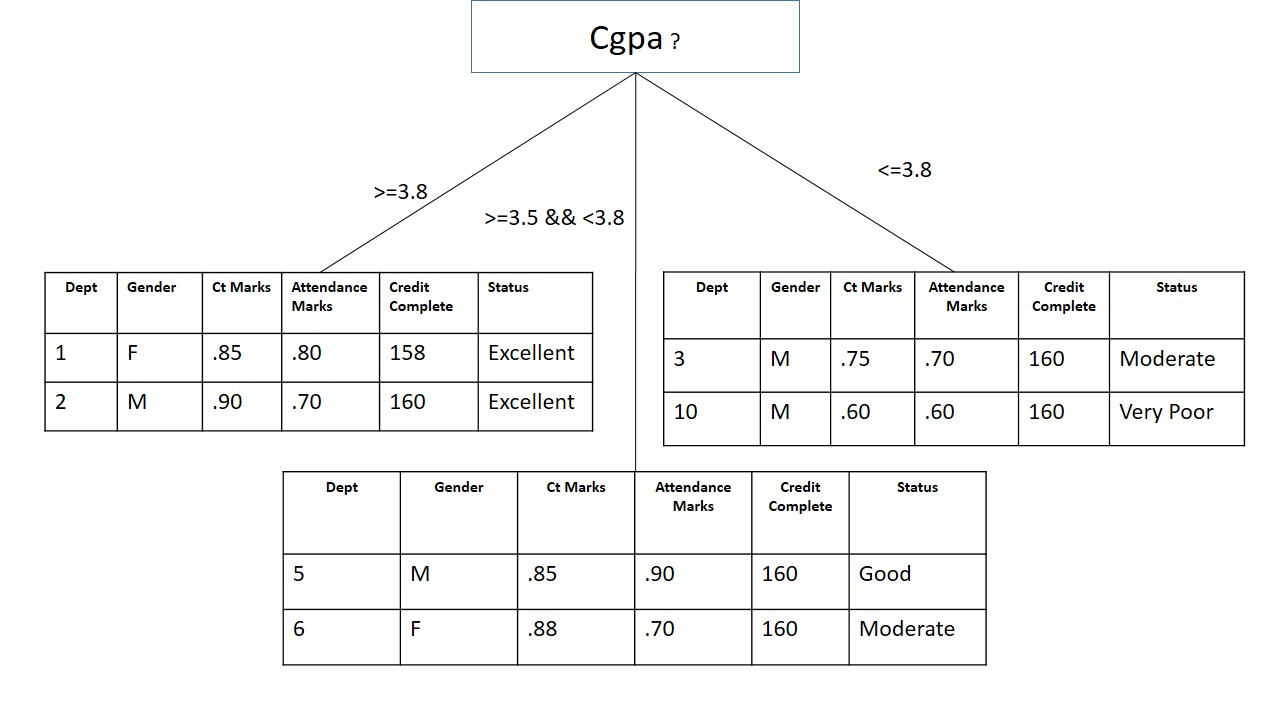
\includegraphics[width=\linewidth]{Figures/Presentation1_2.jpg}
  \decoRule
  \caption[A Decision Tree From Training Data]{A Decision Tree From Training Data}
  \label{fig:Decision Tree From BIIS Training Data}
\end{figure}

\section{Algorithm}
The algorithm used is ID3 Algorithm. So, Information gain as described in Section \ref{infogain} is used as splitting criterion. \\
We used the structure of the algorithm described in Algorithm 1 in our implementation. We used Java programming language for implementation. \\
The pseudocode for the final implementation of the algorithm is shown in Algorithm 2.

{\SetAlgoNoLine
\begin{algorithm}[!ht]

\label{generatedecisiontreeforbiisdata}
\SetKwInOut{Input}{Input}
\SetKwInOut{Output}{Output}

\Input{ \begin{itemize}
\item Data partition, D, which is a set of training tuples and their associated class labels \;
\item $attribute\_list(SID,Dept,Hall,Attendance,CT,Cgpa,CrComplete)$, the set of candidate attributes\;
\item $Attribute\_selection\_method : Information gain with majority voting$.
\end{itemize}}
\Output{A decision tree.}

\begin{algorithmic}[1]
\caption{Generate\_decision\_tree\_For\_BIIS\_Data}
\Procedure{}{}
    \State create a node $N$\;
    \If{tuples in $D$ are all of the same class, $C$,}{
    	return $N$ as leaf node labeled with the class $C$ \;
    }
    
    \If{$attribute\_list$ is empty}{
    	return $N$ as leaf node labeled with the majority class in $D$ \;
    }
   \State apply $Attribute\_selecction\_method(D,attribute\_list)$ to find best splitting\-criterion \;  
        
   \State label node $N$ with $splitting_criterion$ \;
    \If{$splitting\_criterion$ is Dept or Hall\_Status or Gender}
   {
   \State split according to the discrete values of the attribure\;\\
   $ attribute\_list \leftarrow attribute\_list - splitting\_attribute $\;
   } 
  
   \Else
   {
   		\Comment $splitting\_criterion$ is Cgpa or Attendance or Classtest or CreditCompleted. \\
   		\State split 3 ways according to the values of the attribute for example for Cgpa divide at 3.8 and 3.5 into 			3 parts\;\\
   		$ attribute\_list \leftarrow attribute\_list - splitting\_attribute $\;
   } 
      
      \For {each outcome $j$ of $splitting\_criterion$}{
        \State let $D_j$ be the set of data tuples in $D$ satisfying outcome $j$ \; 
        \If{$D_j is empty$}
        {
        	attach a leaf labeled with the majority class in $D$ to node $N$ \;
        }
        \Else {attach a leaf labeled with the majority class in $D$ to node $N$ \;}
	}
\State return $N$ \;
\EndProcedure
\end{algorithmic}
\end{algorithm}}

\section{Result of Classification}
 
\begin{table}
\caption{Test Data Sample}
\label{tab:Test Data Sample}
\centering
\begin{tabular}{|c| c| c| c| c| c|c | c|c }
\toprule
\tabhead{SID} & \tabhead{Dept} & \tabhead{Hall}& \tabhead{Gender}& \tabhead{Attendance}& \tabhead{CT} & \tabhead{Cgpa}& \tabhead{Credit} \\
\midrule
4487	&9&	1&	1	&0.98&	0.77&	3.64&	1\\
4488	&9&	0&	0&	0.72&	0.68&	3.18&	1\\
4489	&9	&0&	0&	0.93&	0.69&	3.49&	1\\
4490	&9	&1	&1	&0.61&	0.59&	3.02&	0.96\\
4492	&11	&1	&1	&0.99&	0.72&	3.06&	0.99\\
4493	&11&	1&	1&	0.71&	0.68&	3.07&	0.91\\
4488	&9	&0	&0	&0.72	&0.68	&3.18&	1\\
4489	&9	&0	&0	&0.93	&0.69	&3.49&	1\\
4490	&9	&1	&1	&0.61	&0.59	&3.02&	0.96\\
4492	&11	&1	&1	&0.99	&0.72	&3.06&	0.99\\
4493	&11	&1	&1	&0.71	&0.68	&3.07&	0.91\\
4494	&11	&1	&0	&0.89	&0.78	&3.25&	0.99\\
4496	&11	&0	&1	&0.98	&0.73	&3.22&	0.99\\


\bottomrule
\end{tabular}
\end{table}


Test data set before applying algorithm looks like Table ~\ref{tab:Test Data Sample}.

\begin{table}
\caption{Final Output Sample}
\label{tab:Final Result}
\centering
\begin{tabular}{|c| c| c| c| c| c|c | c|c|c }
\toprule
\tabhead{SID} & \tabhead{Dept} & \tabhead{Hall}& \tabhead{Gender}& \tabhead{Attendance}& \tabhead{CT} & \tabhead{Cgpa}& \tabhead{Credit} & \tabhead{Status} \\
\midrule
4487	& 9 &	1 &	1	& 0.98 &	0.7 7&	3.64 &	1 & good\\
4488	& 9 &	0 &	0 &	0.72 &	0.68 &	3.18 &	1 & moderate\\
4489	& 9	& 0 &	0 &	0.93 &	0.69 &	3.49 &	1 & good\\
4490	& 9	& 1	& 1	& 0.61 &	0.59 &	3.02 &	0.96 & poor\\
4492	& 11	& 1	& 1	& 0.99 &	0.72 &	3.06 &	0.99 & moderate\\
4493	& 11 &	1 &	1 &	0.71 &	0.68 &	3.07 &	0.91 & poor\\
4488	& 9	& 0	& 0	& 0.72	& 0.68	& 3.18 &	1 & moderate\\
4489	& 9	& 0	& 0	& 0.93	& 0.69	& 3.49 &	1 & good\\
4490	& 9	& 1	& 1	& 0.61	& 0.59	& 3.02 &	0.96 & very poor\\
4492	& 11	& 1	& 1	& 0.99	& 0.72	& 3.06 &	0.99 & poor\\
4493	& 11	& 1	& 1	& 0.71	& 0.68	& 3.07 &	0.91 & very poor\\
4494	& 11	& 1	& 0	& 0.89	& 0.78	& 3.25 &	0.99 & moderate\\
4496	& 11	& 0	& 1	& 0.98	& 0.73	& 3.22 &	0.99 & moderate\\


\bottomrule
\end{tabular}
\end{table}

After applying algortihm as desribed in Algorithm 2 the results as shown in Table \ref{tab:Final Result} are found.

%----------------------------------------------------------------------------------------

\section{Statistical Analysis}

We analyzed the final results and found some relevant statistical results. The categories are\:
\begin{itemize}
\item Department wise performance
\item Impact of gender on performance
\item Impact of hall status on performance
\item Impact of classtest marks on performance
\item Impact of attendance marks on performance
\item Impact of cgpa on performance
\item Impact of credit completion on performance
\end{itemize}
The details of the findings are discussed in Section \ref{resultofanlysis}
%----------------------------------------------------------------------------------------

\section{Result of Statistical Analysis}\label{resultofanlysis}

\subsection{Department wise Performance}
\subsubsection{EEE Department}
The overall performance of EEE department is shown in Figure \ref{fig:Performance of EEE Department}.
\begin{table}
\caption{Performance of EEE department}
\label{tab:eee}
\centering
\begin{tabular}{|c| c| }
\toprule
\tabhead{Class Label} & \tabhead{Percent}\\
\midrule
Excellent & $18\%$\\
Good & $42\%$\\
Moderate & $32\%$\\
Poor & $5\%$\\
Very Poor & $3\%$\\

\bottomrule
\end{tabular}
\end{table}
According to our classifier the percentage of each class label of EEE department is shown in Table \ref{tab:eee}

\begin{figure}
   \centering
  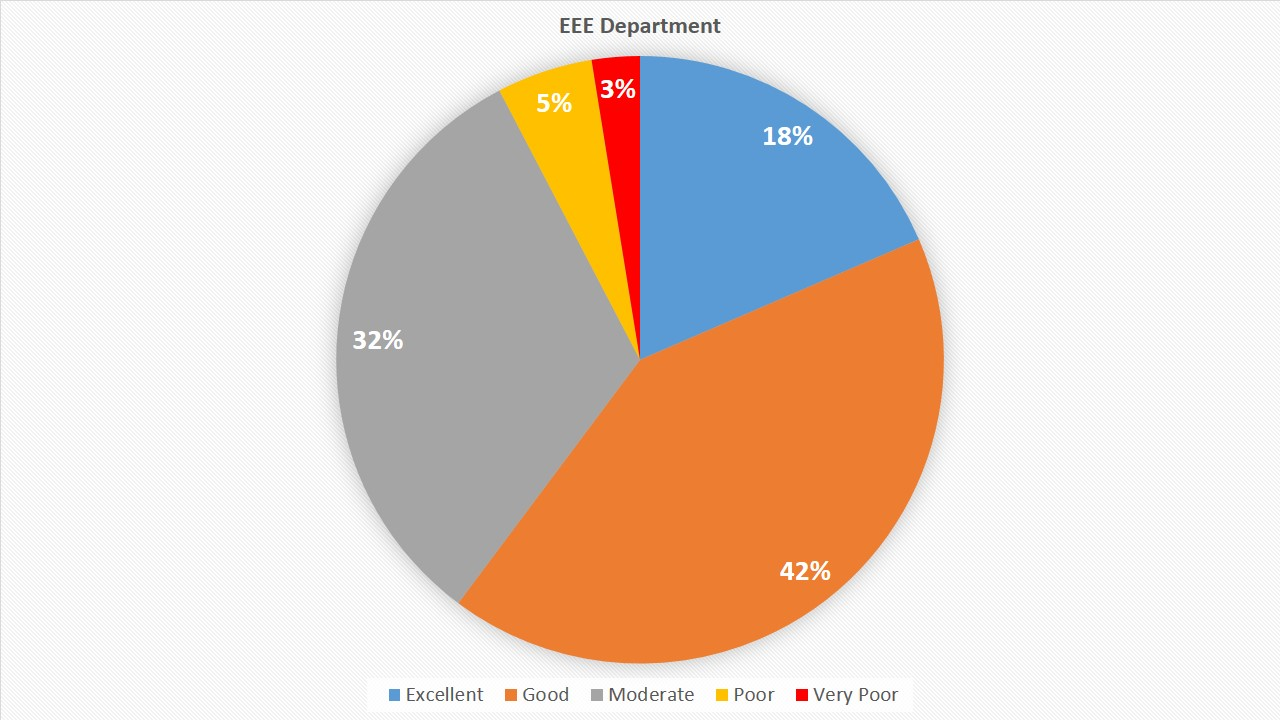
\includegraphics[width=\linewidth]{Figures/Slide3.jpg}
  \decoRule
  \caption[Performance of EEE Department]{Performance of EEE Department}
  \label{fig:Performance of EEE Department}
\end{figure}


\subsubsection{CSE Department}
The overall performance of CSE department is shown in Figure \ref{fig:Performance of CSE Department}.
\begin{table}
\caption{Performance of CSE Department}
\label{tab:cse}
\centering
\begin{tabular}{|c| c| }
\toprule
\tabhead{Class Label} & \tabhead{Percent}\\
\midrule
Excellent & $21\%$\\
Good & $32\%$\\
Moderate & $12\%$\\
Poor & $30\%$\\
Very Poor & $5\%$\\
\bottomrule
\end{tabular}
\end{table}
According to our classifier the percentage of each class label of CSE department is shown in Table \ref{tab:cse}

\begin{figure}
   \centering
  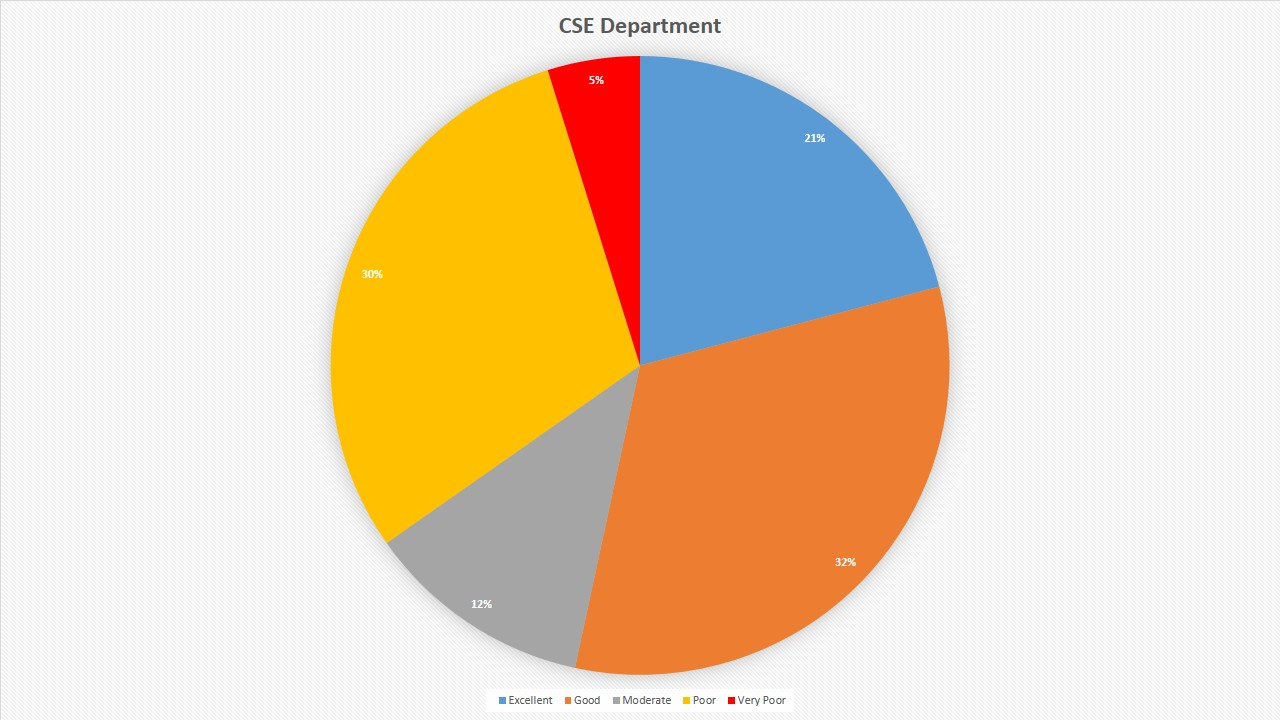
\includegraphics[width=\linewidth]{Figures/Slide2.jpg}
  \decoRule
  \caption[Performance of CSE Department]{Performance of CSE Department}
  \label{fig:Performance of CSE Department}
\end{figure}



\subsubsection{IPE Department}
The overall performance of IPE department is shown in Figure \ref{fig:Performance of IPE Department}.
\begin{table}
\caption{Performance of IPE Department}
\label{tab:ipe}
\centering
\begin{tabular}{|c| c| }
\toprule
\tabhead{Class Label} & \tabhead{Percent}\\
\midrule
Excellent & $13\%$\\
Good & $33\%$\\
Moderate & $17\%$\\
Poor & $23\%$\\
Very Poor & $14\%$\\

\bottomrule
\end{tabular}
\end{table}
According to our classifier the percentage of each class label of IPE department is shown in Table \ref{tab:ipe}

\begin{figure}
   \centering
  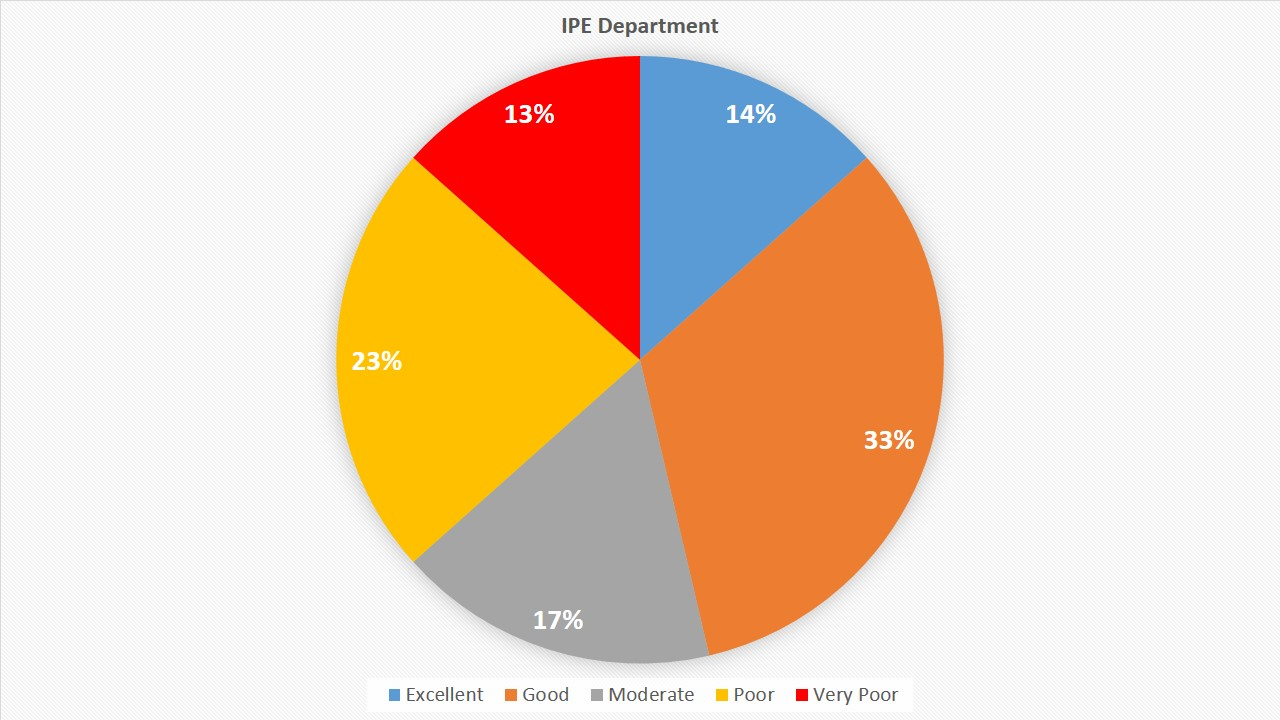
\includegraphics[width=\linewidth]{Figures/Slide4.jpg}
  \decoRule
  \caption[Performance of IPE Department]{Performance of IPE Department}
  \label{fig:Performance of IPE Department}
\end{figure}





\subsubsection{ME Department}
The overall performance of ME department is shown in Figure \ref{fig:Performance of ME Department}.
\begin{table}
\caption{Performance of ME Department}
\label{tab:me}
\centering
\begin{tabular}{|c| c| }
\toprule
\tabhead{Class Label} & \tabhead{Percent}\\
\midrule
Excellent & $5\%$\\
Good & $42\%$\\
Moderate & $37\%$\\
Poor & $6\%$\\
Very Poor & $10\%$\\

\bottomrule
\end{tabular}
\end{table}
According to our classifier the percentage of each class label of ME department is shown in Table \ref{tab:me}

\begin{figure}
   \centering
  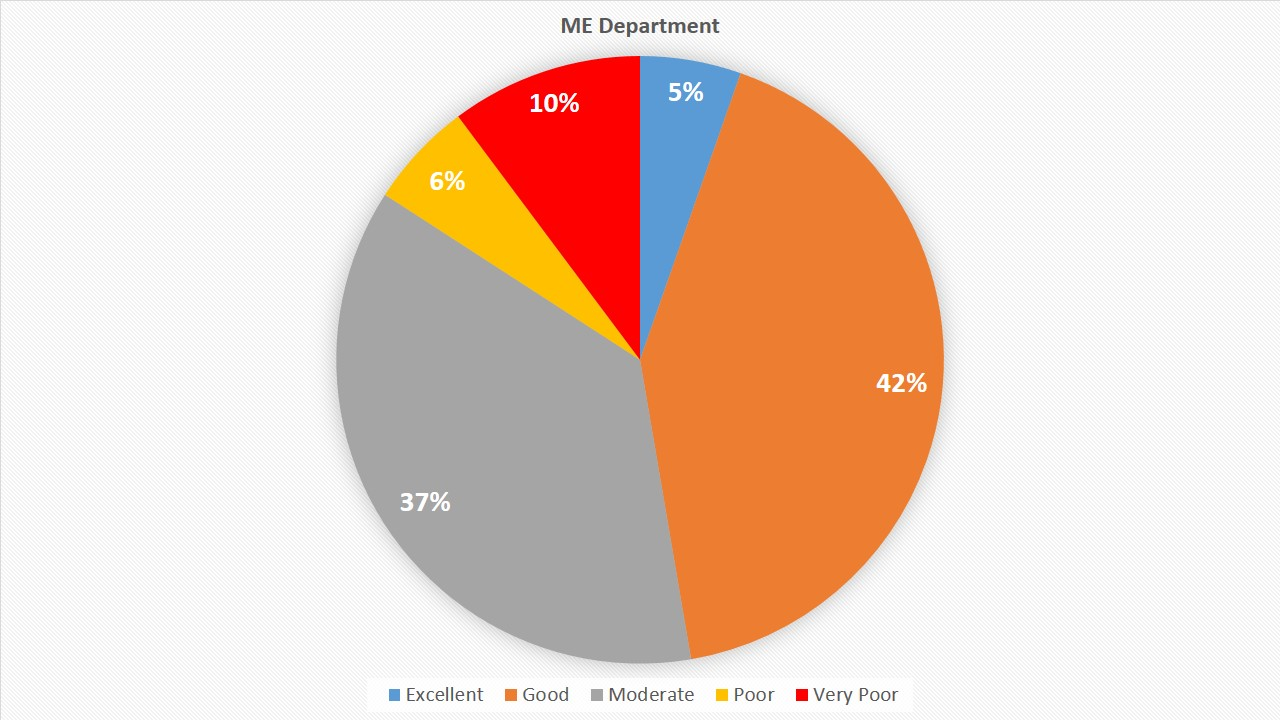
\includegraphics[width=\linewidth]{Figures/Slide5.jpg}
  \decoRule
  \caption[Performance of ME Department]{Performance of ME Department}
  \label{fig:Performance of ME Department}
\end{figure}




\subsubsection{CE Department}
The overall performance of CE department is shown in Figure \ref{fig:Performance of CE Department}.
\begin{table}
\caption{Performance of CE Department}
\label{tab:ce}
\centering
\begin{tabular}{|c| c| }
\toprule
\tabhead{Class Label} & \tabhead{Percent}\\
\midrule
Excellent & $5\%$\\
Good & $27\%$\\
Moderate & $47\%$\\
Poor & $15\%$\\
Very Poor & $6\%$\\

\bottomrule
\end{tabular}
\end{table}
According to our classifier the percentage of each class label of CE department is shown in Table \ref{tab:ce}

\begin{figure}
   \centering
  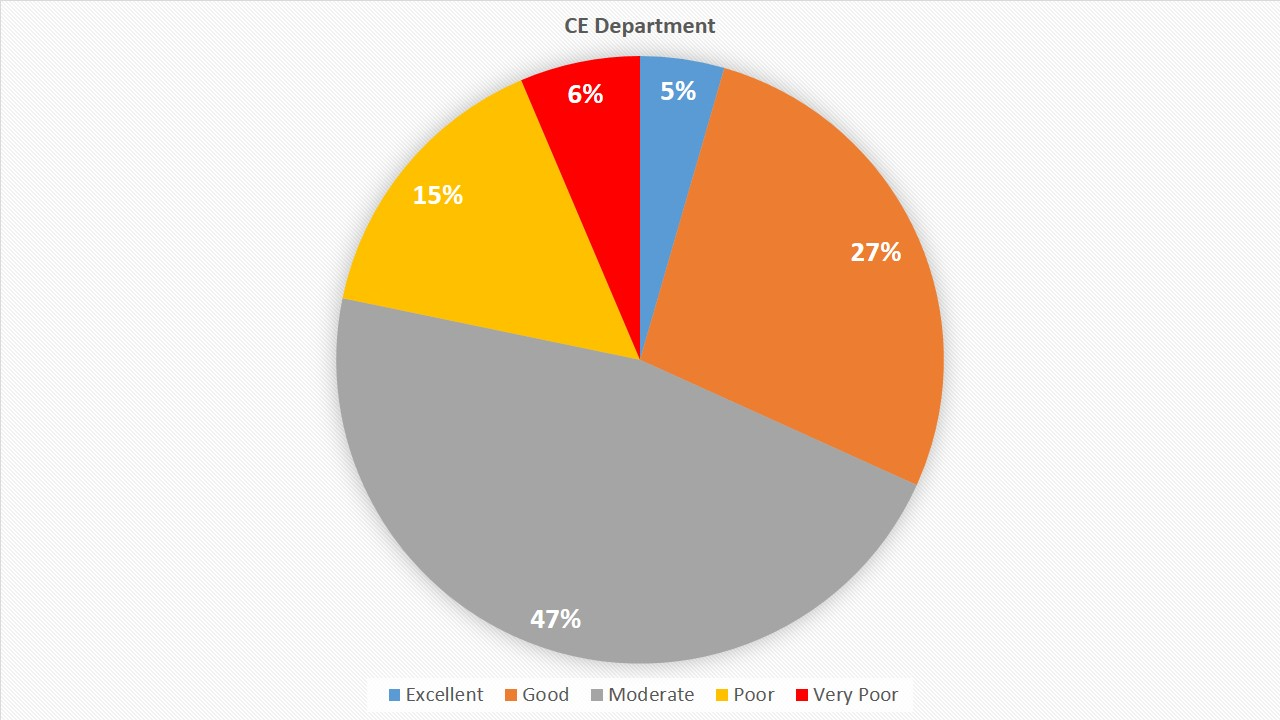
\includegraphics[width=\linewidth]{Figures/Slide6.jpg}
  \decoRule
  \caption[Performance of CE Department]{Performance of CE Department}
  \label{fig:Performance of CE Department}
\end{figure}





\subsubsection{MME Department}
The overall performance of MME department is shown in Figure \ref{fig:Performance of MME Department}.
\begin{table}
\caption{Performance of MME Department}
\label{tab:mme}
\centering
\begin{tabular}{|c| c| }
\toprule
\tabhead{Class Label} & \tabhead{Percent}\\
\midrule
Excellent & $16\%$\\
Good & $37\%$\\
Moderate & $22\%$\\
Poor & $14\%$\\
Very Poor & $11\%$\\
\bottomrule
\end{tabular}
\end{table}
According to our classifier the percentage of each class label of MME department is shown in Table \ref{tab:mme}

\begin{figure}
   \centering
  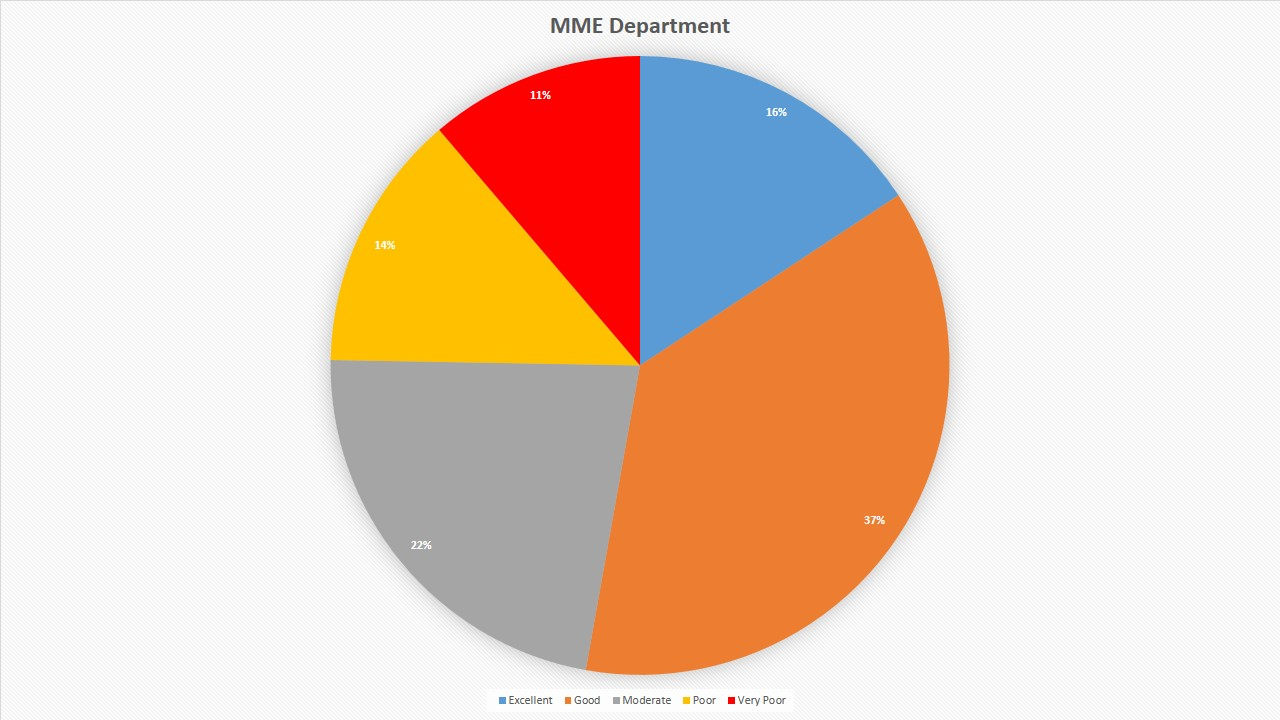
\includegraphics[width=\linewidth]{Figures/Slide7.jpg}
  \decoRule
  \caption[Performance of MME Department]{Performance of MME Department}
  \label{fig:Performance of MME Department}
\end{figure}



\subsubsection{CHE Department}
The overall performance of CHE department is shown in Figure \ref{fig:Performance of CHE Department}.
\begin{table}
\caption{Performance of CHE Department}
\label{tab:che}
\centering
\begin{tabular}{|c| c| }
\toprule
\tabhead{Class Label} & \tabhead{Percent}\\
\midrule
Excellent & $5\%$\\
Good & $62\%$\\
Moderate & $13\%$\\
Poor & $8\%$\\
Very Poor & $12\%$\\

\bottomrule
\end{tabular}
\end{table}
According to our classifier the percentage of each class label of CHE department is shown in Table \ref{tab:che}

\begin{figure}
   \centering
  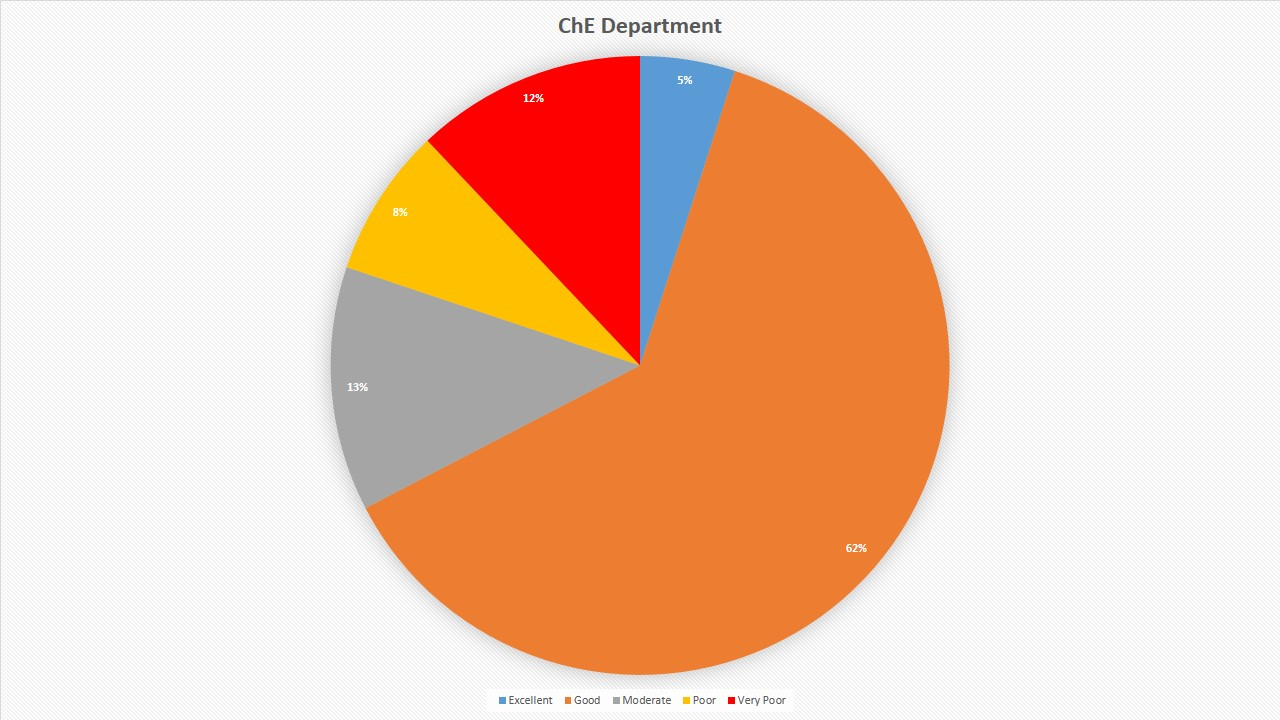
\includegraphics[width=\linewidth]{Figures/Slide8.jpg}
  \decoRule
  \caption[Performance of CHE Department]{Performance of CHE Department}
  \label{fig:Performance of CHE Department}
\end{figure}



\subsubsection{NAME Department}
The overall performance of NAME department is shown in Figure \ref{fig:Performance of NAME Department}.
\begin{table}
\caption{Performance of NAME Department}
\label{tab:name}
\centering
\begin{tabular}{|c| c| }
\toprule
\tabhead{Class Label} & \tabhead{Percent}\\
\midrule
Excellent & $8\%$\\
Good & $48\%$\\
Moderate & $27\%$\\
Poor & $10\%$\\
Very Poor & $7\%$\\

\bottomrule
\end{tabular}
\end{table}
According to our classifier the percentage of each class label of NAME department is shown in Table \ref{tab:name}

\begin{figure}
   \centering
  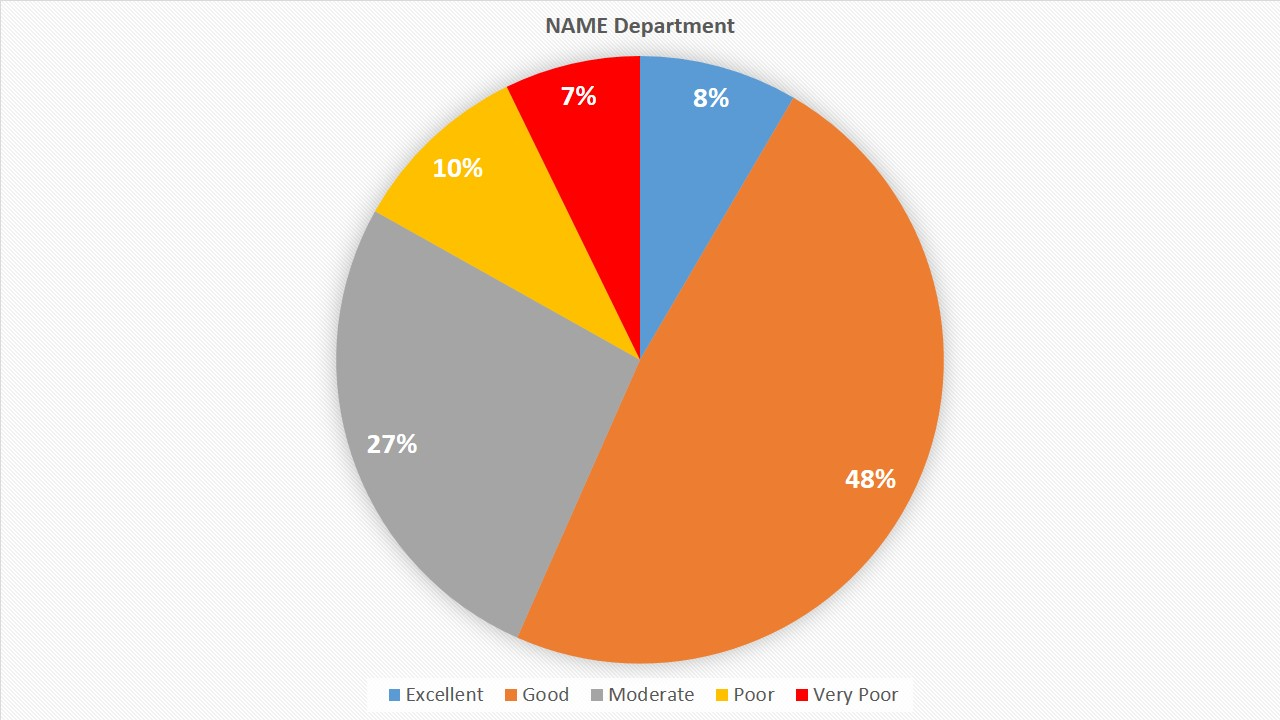
\includegraphics[width=\linewidth]{Figures/Slide9.jpg}
  \decoRule
  \caption[Performance of NAME Department]{Performance of NAME Department}
  \label{fig:Performance of NAME Department}
\end{figure}



\subsubsection{URP Department}
The overall performance of URP department is shown in Figure \ref{fig:Performance of URP Department}.
\begin{table}
\caption{Performance of URP Department}
\label{tab:urp}
\centering
\begin{tabular}{|c| c| }
\toprule
\tabhead{Class Label} & \tabhead{Percent}\\
\midrule
Excellent & $9\%$\\
Good & $40\%$\\
Moderate & $26\%$\\
Poor & $11\%$\\
Very Poor & $14\%$\\

\bottomrule
\end{tabular}
\end{table}
According to our classifier the percentage of each class label of URP department is shown in Table \ref{tab:urp}

\begin{figure}
   \centering
  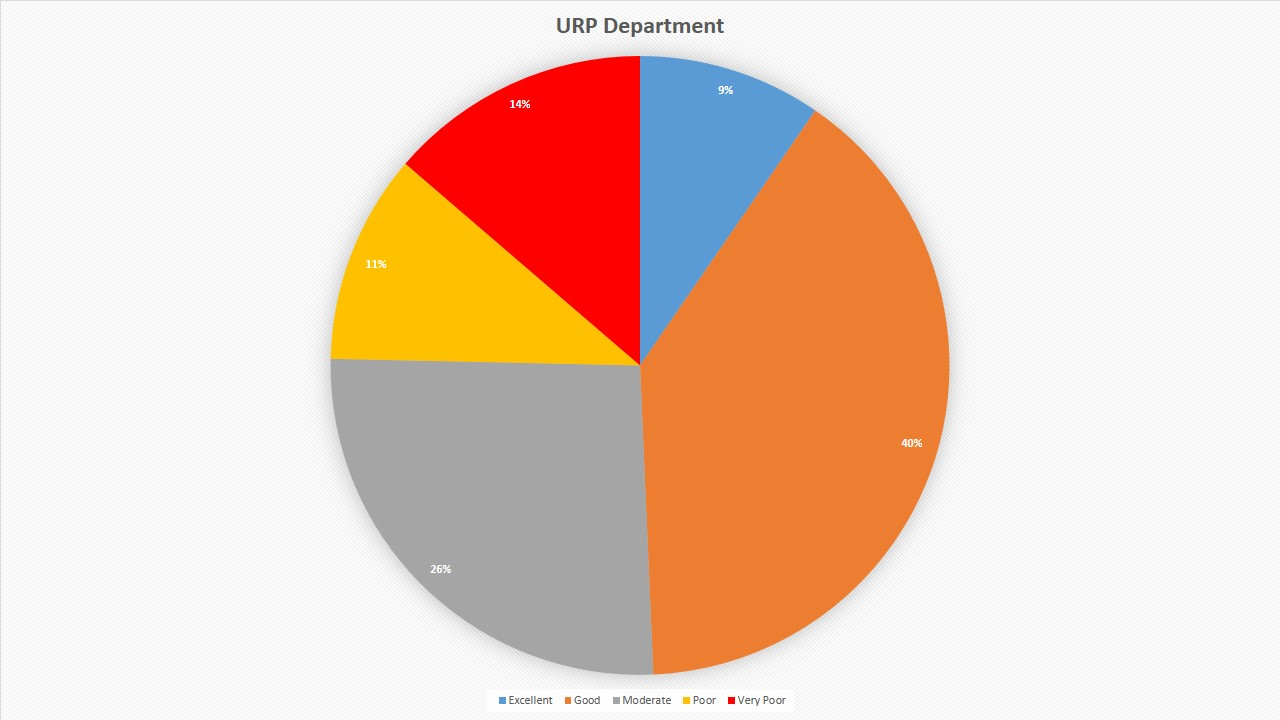
\includegraphics[width=\linewidth]{Figures/Slide10.jpg}
  \decoRule
  \caption[Performance of URP Department]{Performance of URP Department}
  \label{fig:Performance of URP Department}
\end{figure}





\subsubsection{ARCH Department}
The overall performance of ARCH department is shown in Figure \ref{fig:Performance of ARCH Department}.
\begin{table}
\caption{Performance of ARCH Department}
\label{tab:arch}
\centering
\begin{tabular}{|c| c| }
\toprule
\tabhead{Class Label} & \tabhead{Percent}\\
\midrule
Excellent & $2\%$\\
Good & $8\%$\\
Moderate & $32\%$\\
Poor & $16\%$\\
Very Poor & $39\%$\\

\bottomrule
\end{tabular}
\end{table}
According to our classifier the percentage of each class label of ARCH department is shown in Table \ref{tab:arch}

\begin{figure}
   \centering
  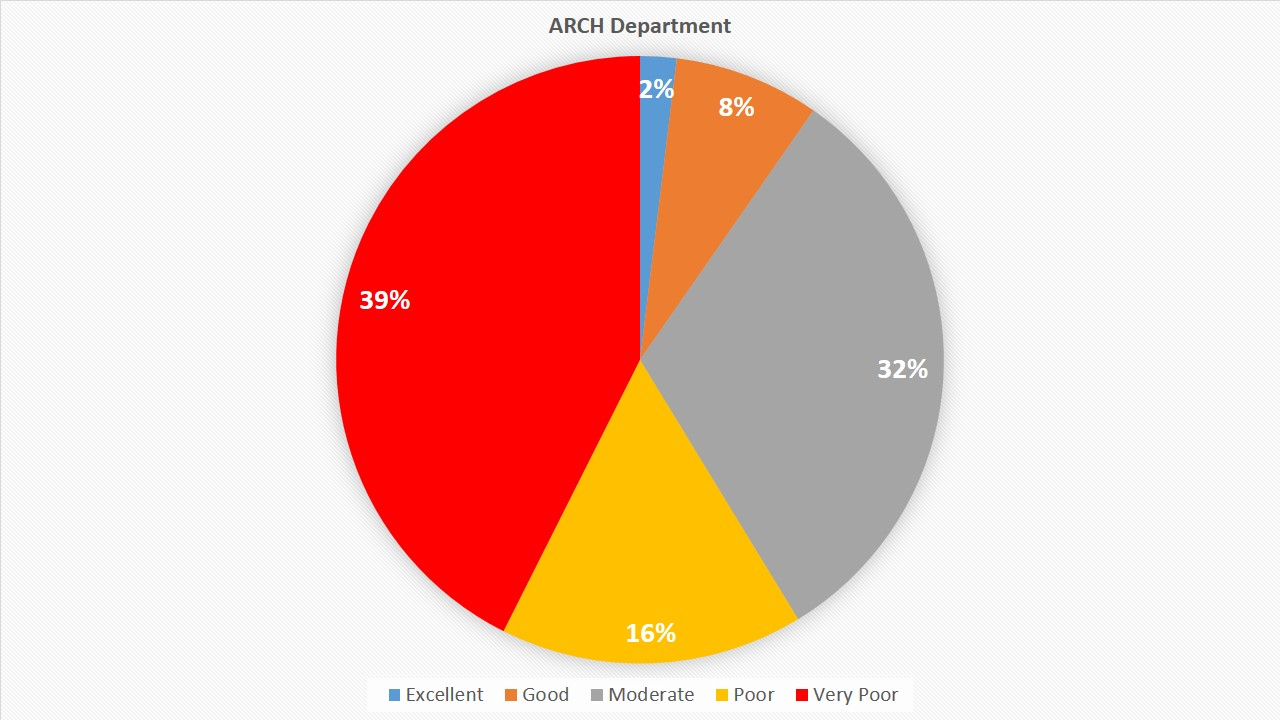
\includegraphics[width=\linewidth]{Figures/Slide11.jpg}
  \decoRule
  \caption[Performance of ARCH Department]{Performance of ARCH Department}
  \label{fig:Performance of ARCH Department}
\end{figure}




\subsubsection{WRE Department}
The overall performance of WRE department is shown in Figure \ref{fig:Performance of WRE Department}.
\begin{table}
\caption{Performance of WRE Department}
\label{tab:wre}
\centering
\begin{tabular}{|c| c| }
\toprule
\tabhead{Class Label} & \tabhead{Percent}\\
\midrule
Excellent & $8\%$\\
Good & $30\%$\\
Moderate & $35\%$\\
Poor & $12\%$\\
Very Poor & $15\%$\\

\bottomrule
\end{tabular}
\end{table}
According to our classifier the percentage of each class label of WRE department is shown in Table \ref{tab:wre}

\begin{figure}
   \centering
  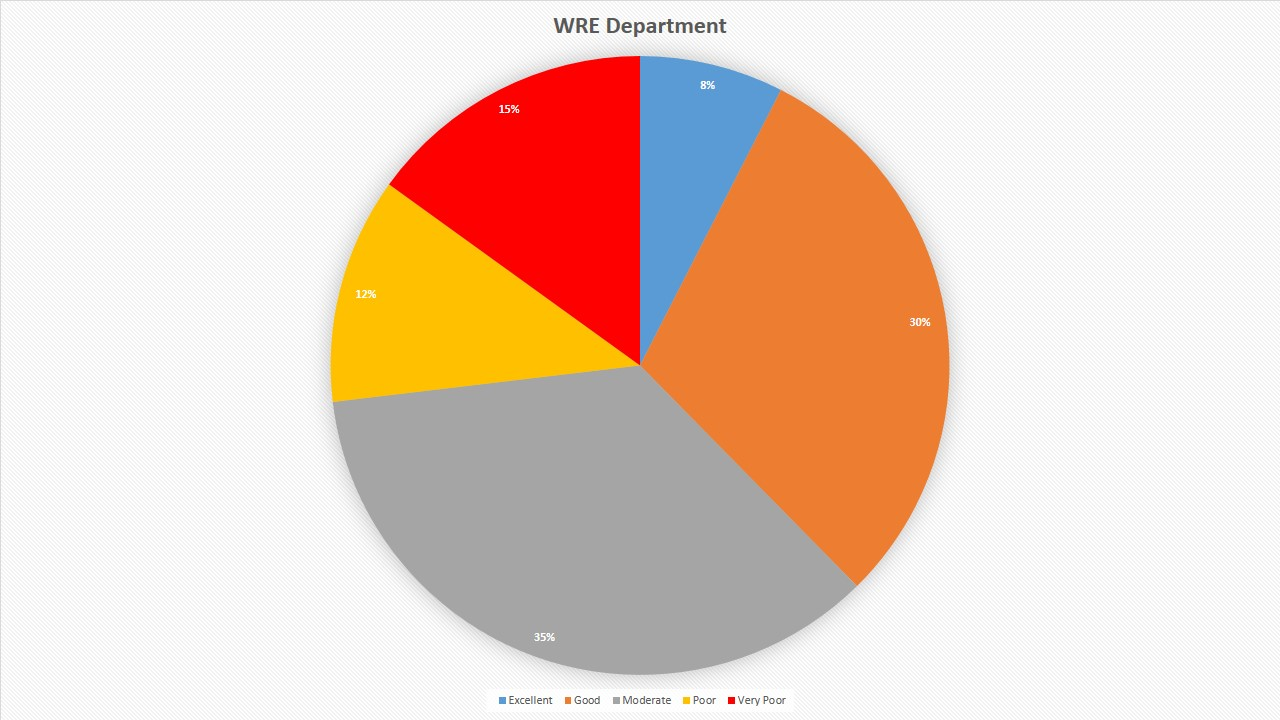
\includegraphics[width=\linewidth]{Figures/Slide12.jpg}
  \decoRule
  \caption[Performance of WRE Department]{Performance of WRE Department}
  \label{fig:Performance of WRE Department}
\end{figure}

\subsubsection{Overall Department wise Performance}
\begin{figure}
   \centering
  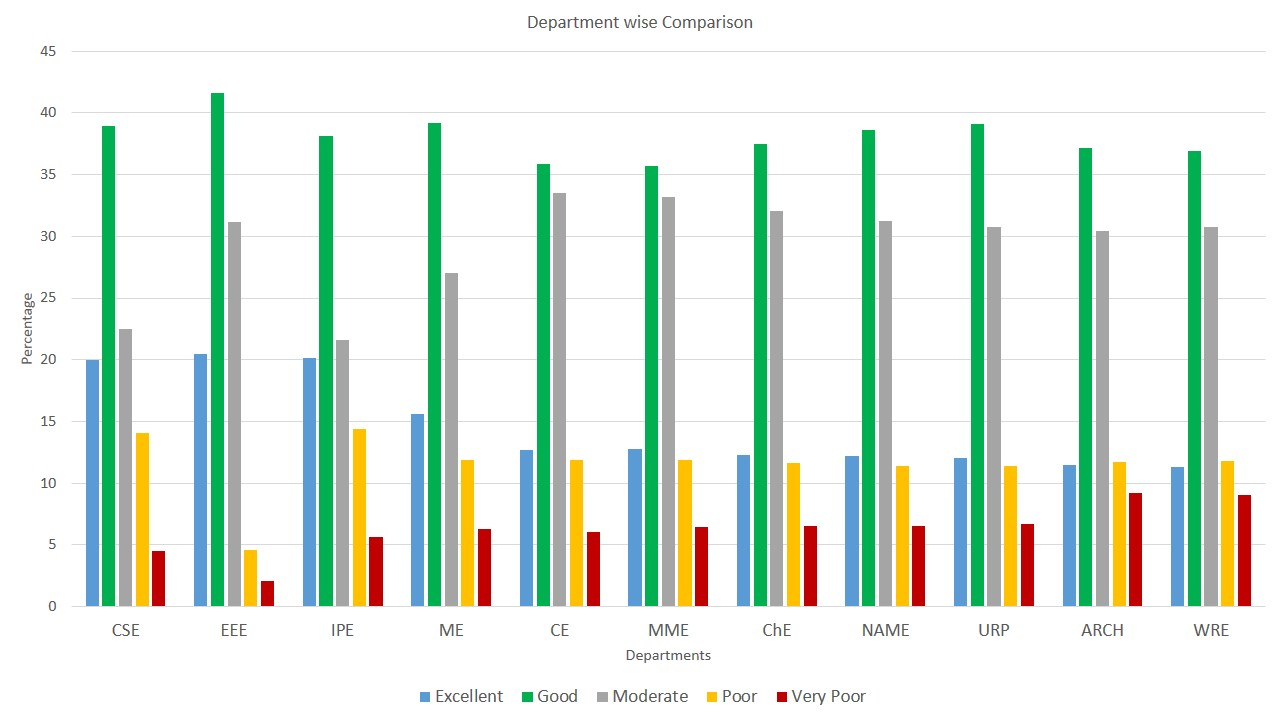
\includegraphics[width=\linewidth]{Figures/Slide19.jpg}
  \decoRule
  \caption[Overall Department wise Performance]{Overall Department wise Performance}
  \label{fig:Overall Department wise Performance}
\end{figure}

Figure \ref{fig:Overall Department wise Performance} shows the overall department wise performance according to our classifier. The amounts are calculated in percentage for better comparison.

\subsection{Impact of Gender on Performance}
Male and female students have different proportion of class label according to our classifier. Female students have higher percentage of their number in  top(excellent) class. In the lowest class(very poor) the percentages are almost equal.Figure \ref{fig:Impact of Gender on Performance} illustrate this phenomena.Table \ref{tab:impactofgender} is the numerical data table for this section.



\begin{figure}
   \centering
  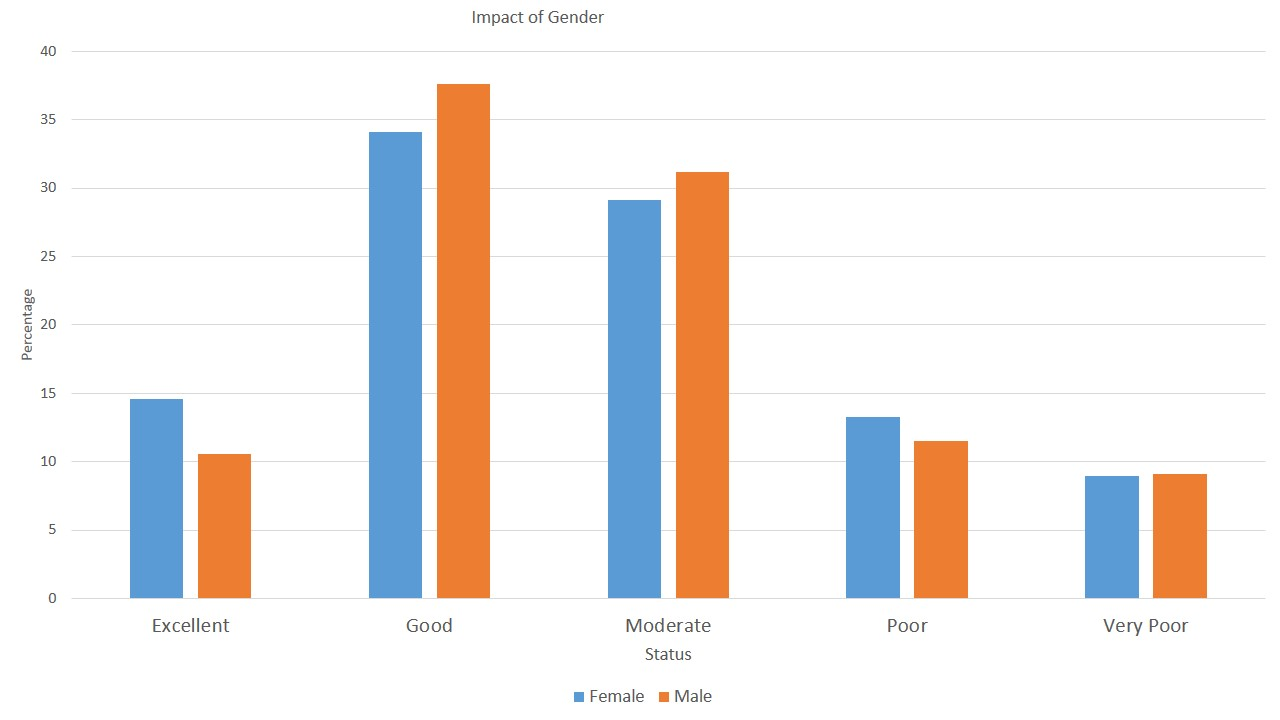
\includegraphics[width=\linewidth]{Figures/Slide13.jpg}
  \decoRule
  \caption[Impact of Gender on Performance]{Impact of Gender on Performance}
  \label{fig:Impact of Gender on Performance}
\end{figure}


\begin{table}
\caption{Impact of Gender on Performance}
\label{tab:impactofgender}
\centering
\begin{tabular}{|c| c|c| }
\toprule
\tabhead{Class Label} & \tabhead{Feale} & \tabhead{Male}\\
\midrule
Excellent	& 14.56\% &	10.55\%\\
Good	& 34.13\% & 	37.59\%\\
Moderate	& 29.13\% &	31.15\%\\
Poor &	13.26 \% &	11.48\%\\
Very Poor &	8.91\% &	9.11\%\\
 
\bottomrule
\end{tabular}
\end{table}

\subsection{Impact of Hall Status on Performance}
Hall status(Resident or Attached) of a student have a profound impact on performance. Attached students have higher percentage of their number in higher classes(excellent,good). In the lower classes the percentages are almost same. Residents are dominant in 'moderate' class. Figure \ref{fig:Impact of Hall Status on Performance} illustrate this phenomena. Table \ref{tab:impactofhall} is the numerical data table for this section.


\begin{figure}
   \centering
  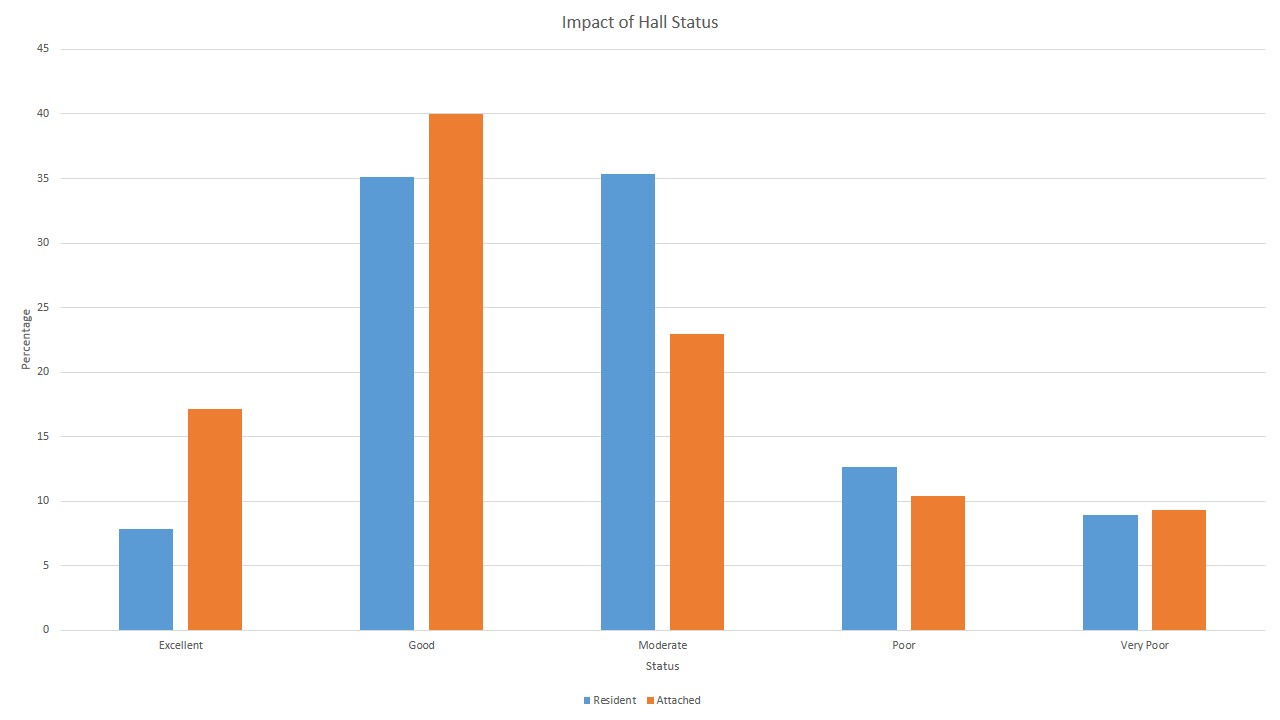
\includegraphics[width=\linewidth]{Figures/Slide14.jpg}
  \decoRule
  \caption[Impact of Hall Status on Performance]{Impact of Hall Status on Performance}
  \label{fig:Impact of Hall Status on Performance}
\end{figure}
 

\begin{table}
\caption{Impact of Hall Status on Performance}
\label{tab:impactofhall}
\centering
\begin{tabular}{|c| c|c| }
\toprule
\tabhead{Class Label} & \tabhead{Resident} & \tabhead{Attached}\\
\midrule
Excellent &	7.88\% &	17.13\%\\
Good	& 35.12\% &	39.97\%\\
Moderate &	35.38\% &	22.95\%\\
Poor	& 12.65\%	& 10.41\%\\
Very Poor &	8.94\% &	9.29\%\\

\bottomrule
\end{tabular}
\end{table} 

 
 
\subsection{Impact of Class Attendance Marks}
Class attendance has a profound impact on a student's performance. Students with high class test marks are tend to be in the higher label. For example students with greater than 90\% attendance is dominant in top class(excellent). On the other hand student with less than 60\% attendance has a very high probability of being in the 'very poor' class. Figure \ref{fig:Impact of Attendance on Performance} describes this phenomena. Table \ref{tab:impactofatt} is the numerical data table for this section.

\begin{figure}
   \centering
  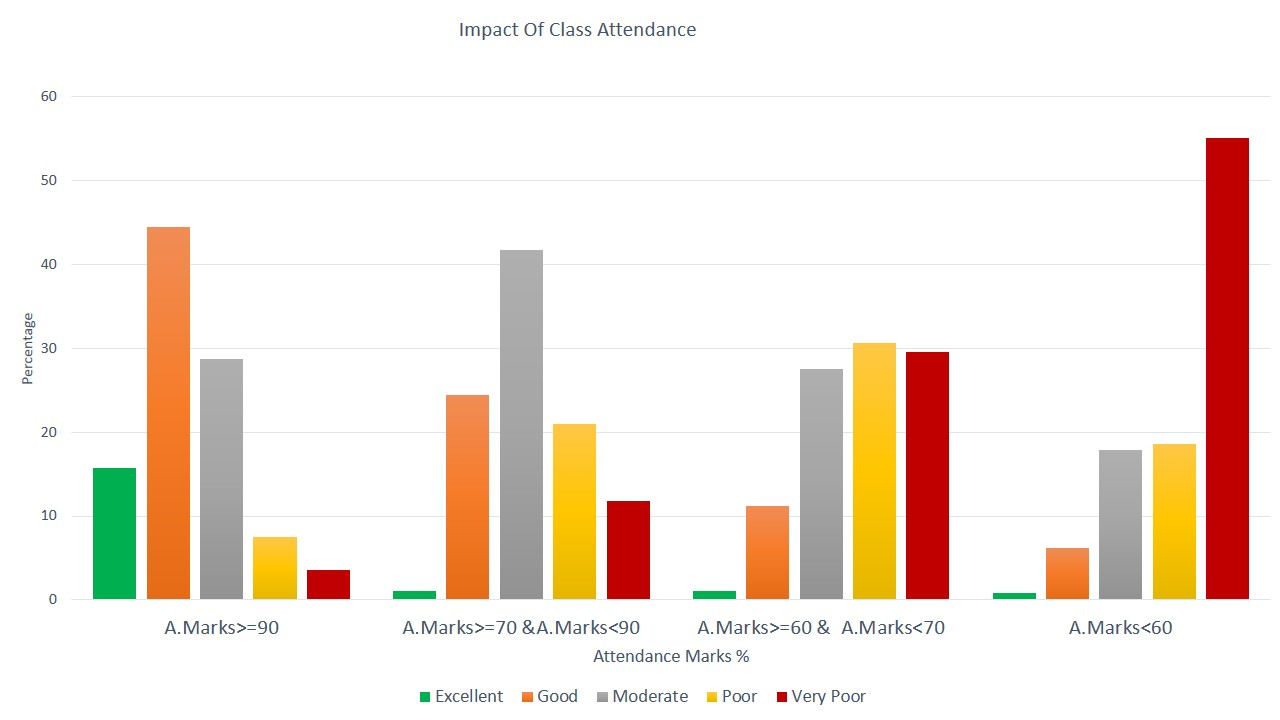
\includegraphics[width=\linewidth]{Figures/Slide15.jpg}
  \decoRule
  \caption[Impact of Attendance on Performance]{Impact of Attendance on Performance}
  \label{fig:Impact of Attendance on Performance}
\end{figure}

\begin{table}
\caption{Impact of Hall Status on Performance}
\label{tab:impactofatt}
\centering
\begin{tabular}{|c| c|c|c|c| }
\toprule
\tabhead{Class Label} & \tabhead{\textgreater 90} & \tabhead{\textgreater 70 and \textless 90 } & \tabhead{ \textgreater 60 and \textless 70 } & \tabhead{\textless 60 }\\
\midrule
Excellent &	15.73\%	& 1.01\%	& 1.02\% &	0.77\% \\
Good	& 44.41\%	& 24.43\% &	11.22\% &	6.20\% \\
Moderate &	28.74\%	 & 41.75\%	& 27.55\%	& 17.82\% \\
Poor	& 7.54\%	& 20.97\%	& 30.61\%	& 18.60\% \\
Very Poor	& 3.56\%	& 11.81\%	& 29.59\%	& 55.03\% \\
\bottomrule
\end{tabular}
\end{table} 
 
\subsection{Impact of Class Test Marks on Performance}
Class test marks plays a very important role on overall performance of a student. Figure \ref{fig:Impact of Class test marks on Performance} shows the result. Table \ref{tab:impactofct} is the data table.

\begin{figure}
   \centering
  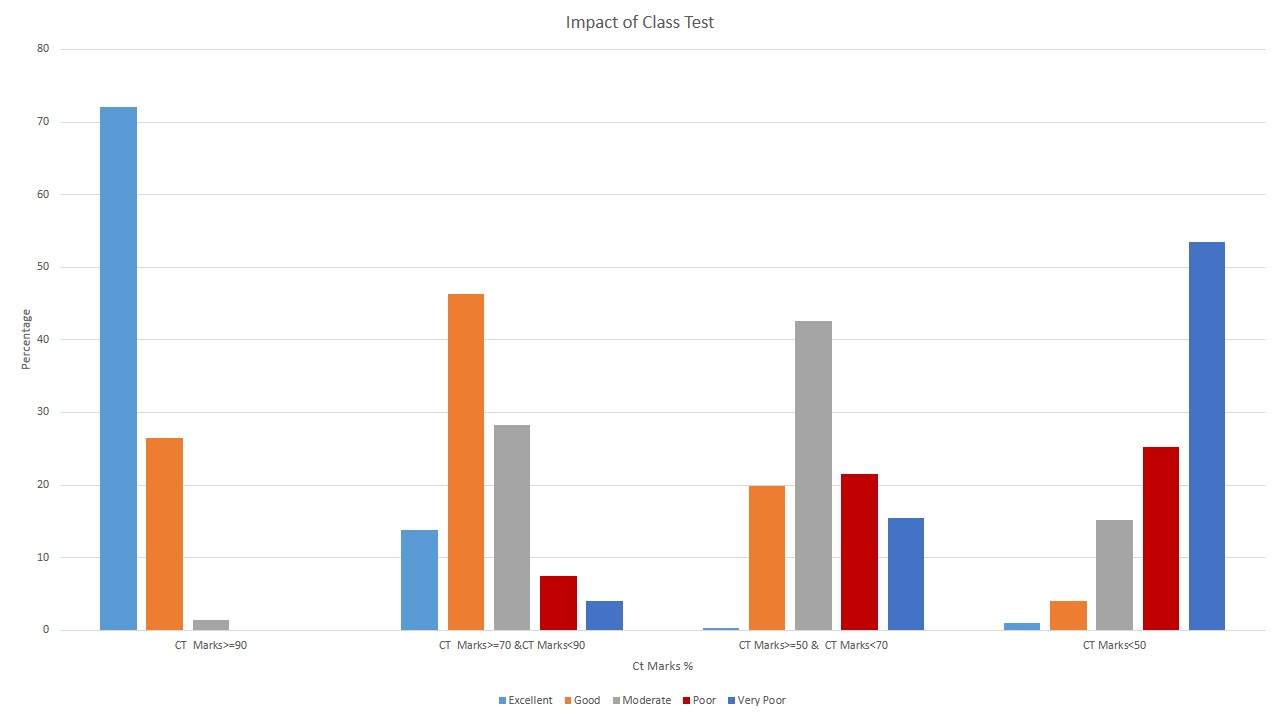
\includegraphics[width=\linewidth]{Figures/Slide16.jpg}
  \decoRule
  \caption[Impact of Class test marks on Performance]{Impact of Class test marks on Performance}
  \label{fig:Impact of Class test marks on Performance}
\end{figure}

\begin{table}
\caption{Impact of Class Test Marks on Performance}
\label{tab:impactofct}
\centering
\begin{tabular}{|c| c|c|c|c| }
\toprule
\tabhead{Class Label} & \tabhead{\textgreater 90} & \tabhead{\textgreater 70 and \textless 90 } & \tabhead{ \textgreater 50 and \textless 70 } & \tabhead{\textless 50 }\\
\midrule
Excellent &	73\%	& 14.1\%	& 1\% &	1\% \\
Good	& 26\%	& 47\% &	20\% &	4\% \\
Moderate &	2\%	 & 29\%	& 43\%	& 15\% \\
Poor	& 0\%	& 8\%	& 22\%	& 26\% \\
Very Poor	& 0\%	& 5\%	& 16\%	& 54\% \\
\bottomrule
\end{tabular}
\end{table} 
 
 
\subsection{Impact of CGPA on Overall Performance}
It is quite obvious that cgpa is the most important part of a student's overall academic performance.
Our classifier also agrees with this fact. About 99\% of the students getting cgpa higher than 3.8 falls in the 'Excellent' class. Those with lower cgpa falls in lower classes.
 
 
\subsection{Impact of Credit Completion}
Completing all the required credit within the regular period of time plays a vital role in overall academic performance. Figure \ref{fig:Impact of Credit completion on Performance} shows the result.\\ \\More statistical analysis results are discussed in Appendix \ref{Appendix B}.

\begin{figure}
   \centering
  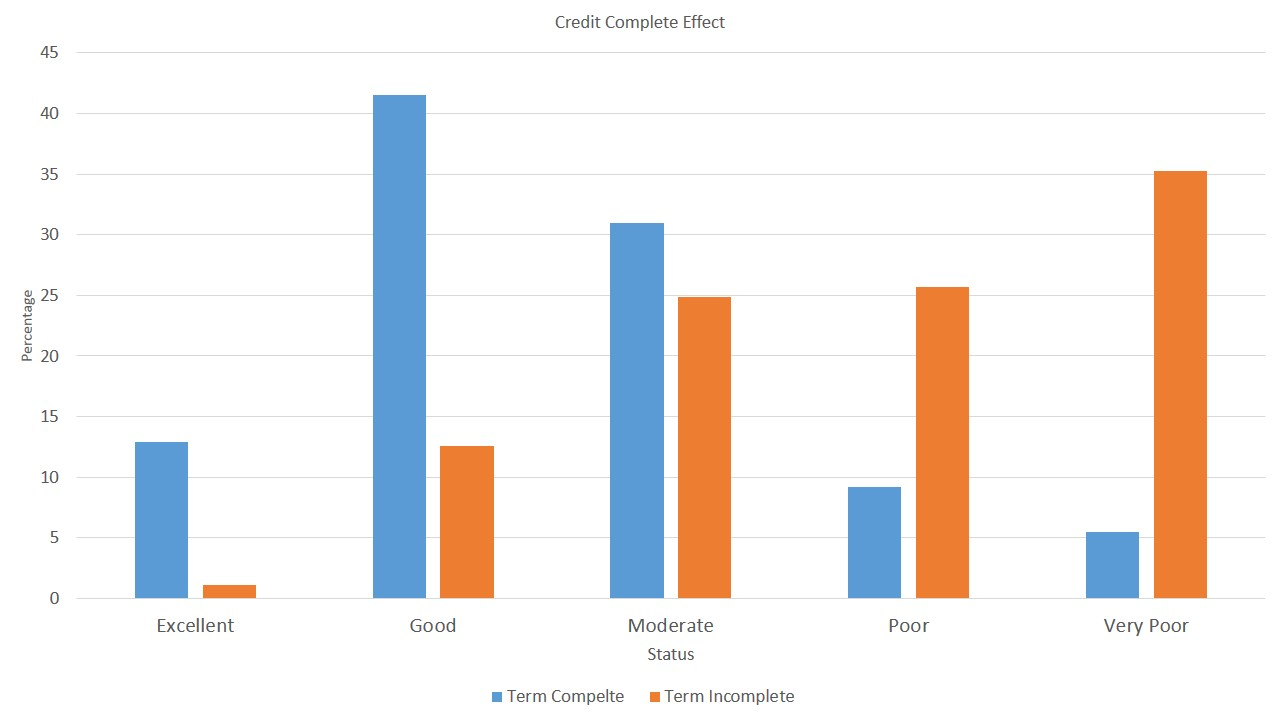
\includegraphics[width=\linewidth]{Figures/Slide18.jpg}
  \decoRule
  \caption[Impact of Credit completion on Performance]{Impact of Credit completion on Performance}
  \label{fig:Impact of Credit completion on Performance}
\end{figure}

 
 